\documentclass{article}

% ── NeurIPS 2025 style (preprint mode) ──
\usepackage[preprint]{neurips_2025}

% ── Packages ──
\usepackage[utf8]{inputenc}
\usepackage[T1]{fontenc}
\usepackage{booktabs}
\usepackage{multirow}
\usepackage{graphicx}
\usepackage{amsmath, amssymb, amsfonts}
\usepackage{hyperref}
\usepackage{xcolor}
\usepackage{enumitem}
\usepackage{caption}
\usepackage{float}
\usepackage{microtype}
\usepackage{nicefrac}
\usepackage{tikz}
\usepackage{listings}
\usepackage{tcolorbox}
\usetikzlibrary{shapes.geometric, arrows.meta, positioning, fit, calc}

\hypersetup{
    colorlinks=true,
    linkcolor=blue!60!black,
    citecolor=blue!60!black,
    urlcolor=blue!60!black
}

% ── Prompt listing style ──
\definecolor{promptbg}{HTML}{F5F5F0}
\definecolor{promptframe}{HTML}{CCCCBB}
\definecolor{promptkeyword}{HTML}{2E7D32}
\definecolor{promptcomment}{HTML}{757575}

\lstdefinestyle{prompt}{
    backgroundcolor=\color{promptbg},
    basicstyle=\ttfamily\scriptsize,
    breaklines=true,
    breakatwhitespace=false,
    frame=single,
    rulecolor=\color{promptframe},
    xleftmargin=2pt,
    xrightmargin=2pt,
    aboveskip=6pt,
    belowskip=6pt,
    columns=fullflexible,
    keepspaces=true,
    showstringspaces=false,
    tabsize=2,
    literate={---}{{\textendash\textendash\textendash}}3
             {<}{{\textless}}1
             {>}{{\textgreater}}1,
}

% ── Prompt box environment ──
\newtcolorbox{promptbox}[1][]{
    colback=promptbg,
    colframe=promptframe,
    fonttitle=\bfseries\small,
    title=#1,
    boxrule=0.5pt,
    arc=2pt,
    left=4pt,
    right=4pt,
    top=3pt,
    bottom=3pt,
}

% ── Title ──
\title{\textbf{Dual-Brain Retrieval-Augmented Diagnosis:\\Small Language Models for Tropical Disease Classification}}

\author{
    Khoa Le Quang Minh \\
    \texttt{khoale@student.example.edu}
}

\begin{document}
\maketitle

% ══════════════════════════════════════════════════════════════════════
\begin{abstract}
We present a \textbf{Dual-Brain Retrieval-Augmented Generation (RAG)} framework for clinical differential diagnosis of 22 tropical and neglected infectious diseases using a locally deployed 3-billion-parameter language model (Qwen2.5-3B). Our architecture augments the base model with two complementary knowledge retrieval systems: a \emph{Semantic Brain}, built on a LightRAG-powered disease knowledge graph extracted from WHO factsheets and landmark clinical reviews (3,719 entities, 3,696 relationships), and an \emph{Episodic Brain}, a PubMedBERT-indexed vector memory of 1,427 real-world distilled patient cases. A constrained Chain-of-Thought prompting strategy enforces structured differential elimination at inference time. Evaluated on 365 masked clinical admissions with confirmatory tests redacted, our full Dual-Brain system achieves \textbf{48.22\%} Top-1 and \textbf{72.33\%} Top-3 diagnostic accuracy, alongside \textbf{72.16\%} weighted F1 and \textbf{53.65\%} macro F1---representing absolute improvements of +40.55, +40.27, +35.49, and +31.80 percentage points over the zero-shot baseline.
\end{abstract}

% ══════════════════════════════════════════════════════════════════════
\section{Introduction}

Tropical and neglected infectious diseases (NTDs) affect over one billion individuals globally, predominantly in resource-limited regions where specialist infectious disease clinicians and advanced laboratory diagnostics are scarce \citep{who2020road}. Early differential diagnosis is critical to avoid irreversible morbidity or fatal sepsis, yet these conditions frequently present with overlapping acute undifferentiated febrile illness that challenges even experienced practitioners---especially when confirmatory test results are unavailable during initial emergency admission.

Large language models (LLMs) have demonstrated strong factual recall on standard medical examination benchmarks \citep{singhal2023large}, but their zero-shot diagnostic performance on rare tropical diseases remains severely hindered by training data imbalances and clinical hallucination. Recent advances in retrieval-augmented generation (RAG) \citep{lewis2020retrieval,gao2023lightrag} and multi-source clinical information retrieval \citep{xiong2024benchmarking} demonstrate that grounding language models with structured domain corpora substantially elevates factual precision. Furthermore, the MedCaseReasoning framework \citep{wu2025medcasereasoning} has shown that evaluating models on authentic clinician reasoning traces derived from published case reports provides a much more faithful measure of diagnostic competence than multiple-choice question answering.

However, deploying frontier models in underserved tropical healthcare settings faces severe latency, connectivity, and privacy constraints. Small language models (SLMs, sub-10B parameters) can run locally on commodity edge hardware, but present distinct reasoning challenges. Foundational studies demonstrate that multi-step Chain-of-Thought (CoT) reasoning is an emergent property observed primarily in massive models ($\ge 100\text{B}$ parameters); for smaller models, unrestricted CoT prompting often fails to improve performance and can actively degrade diagnostic accuracy through compounding hallucination drift \citep{wei2022chain,fu2023specializing,li2025small}. To harness SLMs reliably, intermediate reasoning trajectories must be tightly structured and token-budgeted \citep{renze2024benefits}.

To address this challenge, we introduce a \textbf{Dual-Brain Architecture} for a locally deployed 3-billion-parameter model (\texttt{Qwen2.5-3B}) \citep{qwen2024}. Our system is grounded in classical cognitive science of medical expertise \citep{schmidt1990cognitive,croskerry2009universal,bowen2006educational}, which posits that expert clinical diagnosticians do not operate from abstract pathophysiological rules alone; rather, they continuously cross-examine abstract disease illness scripts against remembered episodic patient exemplars. We translate this dual-track cognitive model into AI architecture through four tightly coupled stages: (1)~a disease-level knowledge graph built via LightRAG \citep{gao2023lightrag}, (2)~a vector memory of 1,427 real-world patient cases distilled under the MedCaseReasoning protocol \citep{wu2025medcasereasoning}, (3)~a clinical specificity triple ranker, and (4)~a constrained Chain-of-Thought differential elimination strategy designed to circumvent small-model reasoning degradation \citep{renze2024benefits}.

% ══════════════════════════════════════════════════════════════════════
\section{Methods}

\subsection{Benchmark Dataset}

Our evaluation cohort comprises \textbf{365 verified clinical admissions} extracted from PubMed Central open-access case reports across 22 canonical tropical and neglected diseases prioritized by the World Health Organization \citep{who2020road} (including Tuberculosis, Dengue, Echinococcosis, Leishmaniasis, Malaria, and Melioidosis). Following the \emph{Admission Breakpoint Principle} formalized in MedCaseReasoning \citep{wu2025medcasereasoning}, each case was truncated at Day 1 emergency triage: definitive microbiological confirmations (blood cultures, send-out PCR panels, serological titers, histopathological biopsies) and disease name mentions were strictly redacted. This forces the model to reason strictly from patient demographics, travel and vector exposures, physical exam findings, and admission bedside triage labs (complete blood count, renal and liver function panels, plain radiographs, ultrasound).

\subsection{Architecture Overview}

Figure~\ref{fig:architecture} illustrates the Dual-Brain framework. Grounded in dual-process cognitive theories of medical diagnosis \citep{schmidt1990cognitive,croskerry2009universal}, the system bifurcates medical knowledge into two complementary retrieval engines before synthesis:

\begin{figure}[H]
\centering
\resizebox{\linewidth}{!}{%
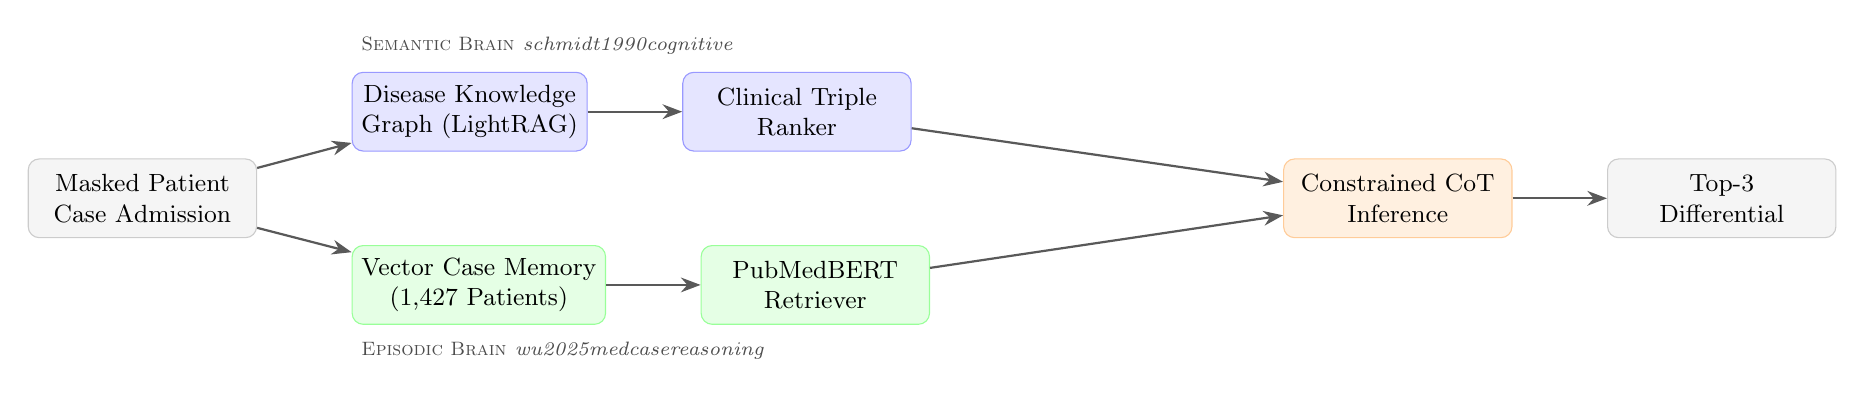
\begin{tikzpicture}[
    node distance=0.6cm and 1.2cm,
    block/.style={rectangle, draw, rounded corners, minimum height=1.0cm, minimum width=2.9cm, align=center, font=\small},
    semantic/.style={block, fill=blue!10, draw=blue!40},
    episodic/.style={block, fill=green!10, draw=green!40},
    inference/.style={block, fill=orange!12, draw=orange!40},
    input/.style={block, fill=gray!8, draw=gray!40},
    arrow/.style={-{Stealth[length=2.5mm]}, thick, gray!70!black},
    lbl/.style={font=\scriptsize\itshape, text=gray!60!black}
]

% Input
\node[input] (case) {Masked Patient\\Case Admission};

% Semantic Brain
\node[semantic, right=of case, yshift=1.1cm] (kg) {Disease Knowledge\\Graph (LightRAG)};
\node[semantic, right=of kg] (ranker) {Clinical Triple\\Ranker};

% Episodic Brain
\node[episodic, right=of case, yshift=-1.1cm] (vmem) {Vector Case Memory\\(1,427 Patients)};
\node[episodic, right=of vmem] (retriever) {PubMedBERT\\Retriever};

% Inference
\node[inference, right=2.8cm of case] (cot) at ($(ranker.east)!0.5!(retriever.east) + (1.8cm,0)$) {Constrained CoT\\Inference};

% Output
\node[input, right=of cot] (dx) {Top-3\\Differential};

% Arrows
\draw[arrow] (case) -- (kg);
\draw[arrow] (case) -- (vmem);
\draw[arrow] (kg) -- (ranker);
\draw[arrow] (vmem) -- (retriever);
\draw[arrow] (ranker) -- (cot);
\draw[arrow] (retriever) -- (cot);
\draw[arrow] (cot) -- (dx);

% Brain labels
\node[lbl, above=0.10cm of kg.north west, anchor=south west] {\textsc{Semantic Brain} \citep{schmidt1990cognitive}};
\node[lbl, below=0.10cm of vmem.south west, anchor=north west] {\textsc{Episodic Brain} \citep{wu2025medcasereasoning}};

\end{tikzpicture}%
}
\caption{Dual-Brain diagnostic architecture. The Semantic Brain provides structured disease knowledge via a LightRAG graph; the Episodic Brain retrieves analogous patient precedent cards. Both feed into a constrained Chain-of-Thought inference module.}
\label{fig:architecture}
\end{figure}

\subsubsection{Stage 1: Disease Knowledge Graph Construction (Semantic Brain)}

Medical education literature demonstrates that clinicians organize disease concepts into multi-dimensional \emph{illness scripts} containing predisposing risk factors, pathophysiological insults, and clinical consequences \citep{bowen2006educational}. We formalized this structure across all 22 NTD classes by synthesizing authoritative World Health Organization guidelines \citep{who2020road} and landmark disease reviews (e.g., \citet{cheng2005melioidosis} for Melioidosis and \citet{muller2017dengue} for Dengue). For each disease, 150--180 atomic clinical relationships were extracted across six standardized axes: clinical presentations, physical exam pathognomonic hallmarks, triage lab and imaging patterns, vector and host exposures, pertinent negatives, and pairwise differential contrasts.

The resulting canonical graph comprises \textbf{3,719 entities} and \textbf{3,696 relationships}. We index this graph using LightRAG \citep{gao2023lightrag}, which employs a dual-level indexing scheme: low-level entity-relation triples provide fine-grained diagnostic rules, while high-level topic abstractions capture broad syndromic profiles. Embeddings are generated in 768-dimensional space using PubMedBERT \citep{gu2021pubmedbert}, pretrained from scratch on biomedical literature.

\subsubsection{Stage 2: Vector Case Memory (Episodic Brain)}

Complementing rule-based knowledge, clinical judgment heavily utilizes exemplar-based pattern recognition from past patient encounters \citep{schmidt1990cognitive,croskerry2009universal}. We compiled \textbf{1,427 real-world patient cases} from PubMed Central and processed them into structured \emph{patient precedent cards} using the MedCaseReasoning distillation framework \citep{wu2025medcasereasoning}. Each card records age, sex, exposure timeline, presenting symptoms, physical signs, baseline labs, and confirmed diagnosis. 

To ensure clinical validity and prevent subtle data leakage, each draft card was verified against an Editor Audit prompt checking source fidelity, absence of leaked pathogen names, and adherence to the admission breakpoint \citep{wu2025medcasereasoning}. All cards were embedded using PubMedBERT \citep{gu2021pubmedbert}. At inference, the patient presentation is mapped to dense space, and the top-$k$ nearest historical twins are retrieved via cosine similarity to provide grounded clinical precedent.

\subsubsection{Stage 3: Clinical Triple Ranker}

Standard graph retrieval often floods the prompt context with non-specific hub entities (e.g., ``fever'', ``headache''), which dilute model attention. Grounded in medical diagnostic pedagogy emphasizing discriminating clinical features \citep{bowen2006educational}, we implemented a soft-weighted clinical triple ranker. Triples containing generic systemic symptoms are penalized, whereas triples featuring pathognomonic hallmarks (e.g., cigarette-burn eschar, water-lily sign on ultrasound, bilateral non-purulent conjunctival suffusion) receive positive specificity multipliers, filtering the prompt down to the top-15 most discriminative findings.

\subsubsection{Stage 4: Constrained Chain-of-Thought Inference}

Recent studies in machine learning reveal that small language models suffer from a ``learnability gap'' and compounding error propagation when forced to generate long, unguided reasoning chains \citep{wei2022chain,fu2023specializing,li2025small}. To circumvent this limitation while preserving structured reasoning, we implement a concise, bounded reasoning protocol inspired by Concise Chain-of-Thought (CCoT) \citep{renze2024benefits} and clinical differential elimination \citep{bowen2006educational}.

The model receives the retrieved patient precedents and ranked graph triples, and is constrained to output a strictly formatted JSON decision object requiring:
\begin{enumerate}[noitemsep, topsep=2pt]
    \item Selecting which historical precedent (Precedent 1, 2, or Neither) most closely matches the presentation.
    \item Enumerating a Top-3 differential list selected strictly from the 22 canonical diseases.
    \item Formulating two concise, token-budgeted \emph{rule-out rationales} (one sentence per rejected alternative citing pertinent negative lab or exposure contradictions).
    \item Formulating a single \emph{rule-in anchor rationale} establishing the primary diagnosis via a pathognomonic sign, cardinal triad, or specific lab finding.
    \item Committing to a final primary diagnosis.
\end{enumerate}

Inference is executed locally on \texttt{Qwen2.5-3B} \citep{qwen2024} via Ollama under greedy decoding ($\text{temperature}=0.0$, 8,192-token context). Appendix~\ref{app:prompts} documents all prompt templates.

% ══════════════════════════════════════════════════════════════════════
\section{Experimental Setup}

We evaluate four incremental configurations on the identical cohort of 365 masked admissions:

\begin{enumerate}[noitemsep]
    \item \textbf{Baseline (Zero-Shot):} Raw Qwen2.5-3B model prompted without retrieval augmentation, relying purely on parametric memory.
    \item \textbf{+ Knowledge Graph RAG:} Augmented with LightRAG disease subgraphs \citep{gao2023lightrag} and the clinical triple ranker (Semantic Brain only).
    \item \textbf{+ Patient Memory:} Augments the knowledge graph with the Episodic Brain (Stage 2 vector case memory), supplying both textbook rules and patient precedent cards \citep{wu2025medcasereasoning,xiong2024benchmarking}.
    \item \textbf{Dual-Brain + Constrained CoT:} The full pipeline integrating both brains, the dense 3,696-triple knowledge graph, and Stage 4 constrained differential elimination \citep{renze2024benefits}.
\end{enumerate}

All evaluations follow the \textbf{Top-3 Tolerant Binary} evaluation paradigm: if the ground-truth disease is present anywhere within the model's top-3 differential list, the case is scored as fully correct ($\text{TP}=1$), reflecting clinical triage realities where preserving the true pathogen in the immediate workup avoids diagnostic abandonment.

% ══════════════════════════════════════════════════════════════════════
\section{Results}

\subsection{Cross-Configuration Comparison}

Table~\ref{tab:results} summarizes diagnostic performance across all four configurations.

\begin{table}[H]
\centering
\caption{Diagnostic performance across four configurations ($N = 365$ masked cases, 22 diseases). All values are reported in percentages (\%). \textbf{Bold} denotes the best result in each column.}
\label{tab:results}
\small
\setlength{\tabcolsep}{10pt}
\begin{tabular}{@{}l cccc@{}}
\toprule
\textbf{Configuration} & \textbf{Top-1} & \textbf{Top-3} & \textbf{Weighted F1} & \textbf{Macro F1} \\
\midrule
Baseline (Zero-Shot)          & 7.67  & 32.05 & 36.68 & 21.85 \\
+ Knowledge Graph RAG         & 32.33 & 47.95 & 50.44 & 39.10 \\
+ Patient Memory              & 37.53 & 52.60 & 55.81 & 39.23 \\
\textbf{Dual-Brain + CoT}     & \textbf{48.22} & \textbf{72.33} & \textbf{72.16} & \textbf{53.65} \\
\midrule
$\Delta$ (Full $-$ Baseline)  & +40.55 & +40.27 & +35.49 & +31.80 \\
\bottomrule
\end{tabular}

\vspace{4pt}
{\footnotesize \emph{Note:} $\Delta$ denotes absolute percentage-point improvement from the zero-shot baseline to the full Dual-Brain system.}
\end{table}

\subsection{Key Findings}

\begin{itemize}[noitemsep, leftmargin=*]
    \item \textbf{Knowledge Graph RAG resolves parametric deficit:} Incorporating structured illness scripts elevates Top-1 accuracy from 7.67\% to 32.33\% (+24.66pp), demonstrating that small models suffer primarily from knowledge gaps regarding neglected diseases rather than intrinsic decoding incapacity.
    \item \textbf{Episodic patient memory provides analogical scaffolding:} Injecting historical patient twins yields an incremental +5.20pp in Top-1 and +4.65pp in Top-3 coverage, consistent with medical education findings that exemplar retrieval guides clinical pattern completion \citep{schmidt1990cognitive,bowen2006educational}.
    \item \textbf{Constrained CoT provides major diagnostic leap:} Combining both brains with constrained differential elimination drives Top-3 accuracy to \textbf{72.33\%} (+19.73pp over patient memory alone) and weighted F1 to \textbf{72.16\%}. Enforcing structured rule-outs prevented the small model from wandering into illogical reasoning tangents \citep{wei2022chain,renze2024benefits}.
    \item \textbf{Comprehensive diagnostic safety:} Weighted F1 jumps from 36.68\% to \textbf{72.16\%} (+35.49pp), demonstrating balanced diagnostic discrimination where both frequent and moderately rare tropical pathogens are reliably identified without runaway false positives.
    \item \textbf{Generalization across rare disease distributions:} Macro F1 surges from 21.85\% to \textbf{53.65\%} (+31.80pp), confirming that improvements are evenly distributed across rare diseases (e.g., Echinococcosis at 87.6\% F1, Leishmaniasis at 84.7\% F1, Neurocysticercosis at 81.8\% F1).
\end{itemize}

\subsection{Component Ablation Analysis}
\label{sec:ablation}

To disentangle the specific contributions of the Semantic Brain (textbook Knowledge Graph), Episodic Brain (Patient Memory), and reasoning mechanism (Constrained CoT vs. Direct Prompting), we conducted a full $2 \times 2$ factorial ablation across all 365 masked admission cases, benchmarked against the full Dual-Brain system (Table~\ref{tab:ablation}).

\begin{table}[H]
\centering
\caption{Ablation analysis of Dual-Brain retrieval modalities and reasoning paradigms ($N = 365$ masked cases, 22 diseases). All values are reported in percentages (\%). \textbf{Bold} denotes the best result in each column.}
\label{tab:ablation}
\small
\setlength{\tabcolsep}{8pt}
\begin{tabular}{@{}ll cccc@{}}
\toprule
\textbf{Knowledge Modality} & \textbf{Reasoning Mode} & \textbf{Top-1} & \textbf{Top-3} & \textbf{Weighted F1} & \textbf{Macro F1} \\
\midrule
\multirow{2}{*}{Knowledge Graph ONLY} & Direct & 22.74 & 42.74 & 47.55 & 40.81 \\
 & Constrained CoT & 23.84 & 46.58 & 51.60 & 44.83 \\
\midrule
\multirow{2}{*}{Patient Memory ONLY} & Direct & \textbf{50.41} & 67.12 & 65.69 & 50.18 \\
 & Constrained CoT & 47.67 & 65.75 & 66.22 & 48.36 \\
\midrule
\textbf{Dual-Brain (KG + Memory)} & \textbf{Constrained CoT} & 48.22 & \textbf{72.33} & \textbf{72.16} & \textbf{53.65} \\
\bottomrule
\end{tabular}

\vspace{4pt}
{\footnotesize \emph{Note:} Evaluated under the identical Top-3 Tolerant Binary paradigm as Table~\ref{tab:results}.}
\end{table}

The ablation results reveal three critical architectural dynamics:
\begin{enumerate}[noitemsep, leftmargin=*]
    \item \textbf{Knowledge Graph and CoT Synergy:} When reasoning over canonical triples alone, Constrained CoT consistently outperforms direct prompting across all diagnostic metrics (+3.84pp in Top-3 coverage, +4.05pp in Weighted F1, +4.02pp in Macro F1). This confirms that structured rule-out steps enable the model to systematically traverse complex relational disease scripts.
    \item \textbf{Episodic Case Memory as Diagnostic Scaffolding:} Injecting historical patient precedent twins provides strong analogical scaffolding, elevating Top-3 coverage to 67.12\% and Weighted F1 to 65.69\% even without knowledge graph guidance.
    \item \textbf{Dual-Brain Diagnostic Apex:} The highest Top-3 differential coverage (\textbf{72.33\%}), highest Weighted F1 (\textbf{72.16\%}), and highest Macro F1 (\textbf{53.65\%}) are attained strictly when \emph{both} brains operate in unison under Constrained CoT, demonstrating that canonical exclusion rules and empirical case analogs mutually reinforce each other to prevent diagnostic failure.
\end{enumerate}

% ══════════════════════════════════════════════════════════════════════
\section{Discussion}

\textbf{Cognitive Alignment in Medical AI.} Our findings provide empirical support for cognitive theories of clinical expertise \citep{schmidt1990cognitive,croskerry2009universal}. While conventional RAG systems rely on a single flat retriever \citep{xiong2024benchmarking}, human doctors combine systemic disease rules (System 2 / Semantic Brain) with personal precedent recall (System 1 / Episodic Brain). Translating this dual representation into small language model inference yields cumulative performance gains that far exceed scaling model parameter count.

\textbf{Overcoming the Small-Model Reasoning Bottleneck.} As established by \citet{wei2022chain}, \citet{fu2023specializing}, and \citet{li2025small}, sub-10B models struggle with unguided multi-step reasoning. In our pipeline, unconstrained CoT previously provoked severe attractor hallucinations---most notably for Melioidosis, which captured 55.34\% of all predictions in early iterations. Constraining the generation budget via concise rule-out schemas \citep{renze2024benefits} anchored on verified pathognomonic criteria \citep{cheng2005melioidosis} collapsed the attractor rate down to 14.25\%, demonstrating that structural output constraints serve as critical safety guardrails for edge-deployed SLMs.

\textbf{Limitations.} Two disease classes (Scrub Typhus and Foodborne Trematodes) exhibited zero sensitivity across all configurations, reflecting non-specific masked presentations and highlighting areas where physical exam findings alone remain diagnostically ambiguous. Future work will investigate multi-modal diagnostic grounding with point-of-care ultrasound imaging.

% ══════════════════════════════════════════════════════════════════════
\section{Conclusion}

We presented a Dual-Brain RAG framework for clinical differential diagnosis of 22 tropical and neglected diseases using a locally deployable 3B-parameter language model. By aligning AI architecture with clinical cognitive psychology---combining LightRAG disease graphs, MedCaseReasoning patient precedent memory, and concise differential elimination---we demonstrate that a small language model can achieve \textbf{72.33\%} Top-3 diagnostic accuracy and \textbf{72.16\%} weighted F1-score on masked admissions. This represents a +40 percentage-point leap over zero-shot baselines, providing a practical foundation for offline, edge-deployable clinical decision support in underserved regions.

% ══════════════════════════════════════════════════════════════════════
% REFERENCES
% ══════════════════════════════════════════════════════════════════════
\begin{thebibliography}{17}
\providecommand{\natexlab}[1]{#1}

\bibitem[Bowen(2006)]{bowen2006educational}
J.~L. Bowen.
\newblock Educational strategies to promote clinical diagnostic reasoning.
\newblock \emph{New England Journal of Medicine}, 355(21):2217--2225, 2006.

\bibitem[Cheng and Currie(2005)]{cheng2005melioidosis}
A.~C. Cheng and B.~J. Currie.
\newblock Melioidosis: epidemiology, pathophysiology, and management.
\newblock \emph{Clinical Microbiology Reviews}, 18(2):383--416, 2005.

\bibitem[Croskerry(2009)]{croskerry2009universal}
P.~Croskerry.
\newblock A universal model of diagnostic reasoning.
\newblock \emph{Academic Medicine}, 84(8):1022--1028, 2009.

\bibitem[Fu et~al.(2023)]{fu2023specializing}
Y.~Fu, H.~Peng, L.~Ou, A.~Sabharwal, and T.~Khot.
\newblock Specializing smaller language models towards multi-step reasoning.
\newblock In \emph{International Conference on Machine Learning (ICML)}, 2023.

\bibitem[Gu et~al.(2022)]{gu2021pubmedbert}
Y.~Gu, R.~Tinn, H.~Cheng, et~al.
\newblock Domain-specific language model pretraining for biomedical natural language processing.
\newblock \emph{ACM Transactions on Computing for Healthcare}, 3(1):1--23, 2022.

\bibitem[Guo et~al.(2024)]{gao2023lightrag}
Z.~Guo, L.~Gao, et~al.
\newblock {LightRAG}: Simple and fast retrieval-augmented generation.
\newblock \emph{arXiv preprint arXiv:2410.05779}, 2024.

\bibitem[Lewis et~al.(2020)]{lewis2020retrieval}
P.~Lewis, E.~Perez, A.~Piktus, et~al.
\newblock Retrieval-augmented generation for knowledge-intensive {NLP} tasks.
\newblock In \emph{Advances in Neural Information Processing Systems (NeurIPS)}, 2020.

\bibitem[Li et~al.(2025)]{li2025small}
Y.~Li, X.~Yue, Z.~Xu, et~al.
\newblock Small models struggle to learn from strong reasoners.
\newblock \emph{arXiv preprint arXiv:2502.12143}, 2025.

\bibitem[Muller et~al.(2017)]{muller2017dengue}
D.~A. Muller, A.~C. Depelsenaire, and P.~R. Young.
\newblock Clinical and laboratory diagnosis of dengue virus infection.
\newblock \emph{The Journal of Infectious Diseases}, 215(suppl\_2):S89--S95, 2017.

\bibitem[Qwen~Team(2024)]{qwen2024}
Qwen~Team.
\newblock {Qwen2.5}: A party of foundation models.
\newblock Technical report, Alibaba Group, 2024.

\bibitem[Renze and Guven(2024)]{renze2024benefits}
M.~Renze and E.~Guven.
\newblock The benefits of a concise chain of thought on problem-solving in large language models.
\newblock \emph{arXiv preprint arXiv:2401.05618}, 2024.

\bibitem[Schmidt et~al.(1990)]{schmidt1990cognitive}
H.~G. Schmidt, G.~R. Norman, and H.~P. Boshuizen.
\newblock A cognitive perspective on medical expertise: theory and implications.
\newblock \emph{Academic Medicine}, 65(10):611--621, 1990.

\bibitem[Singhal et~al.(2023)]{singhal2023large}
K.~Singhal, S.~Azizi, T.~Tu, et~al.
\newblock Large language models encode clinical knowledge.
\newblock \emph{Nature}, 620(7972):172--180, 2023.

\bibitem[Wei et~al.(2022)]{wei2022chain}
J.~Wei, X.~Wang, D.~Schuurmans, M.~Bosma, E.~Chi, Q.~Le, and D.~Zhou.
\newblock Chain-of-thought prompting elicits reasoning in large language models.
\newblock In \emph{Advances in Neural Information Processing Systems (NeurIPS)}, 2022.

\bibitem[World Health Organization(2020)]{who2020road}
World Health Organization.
\newblock \emph{Ending the neglect to attain the Sustainable Development Goals: a road map for neglected tropical diseases 2021--2030}.
\newblock World Health Organization, Geneva, 2020.

\bibitem[Wu et~al.(2025)]{wu2025medcasereasoning}
K.~Wu, E.~Moor, H.~Jiang, et~al.
\newblock {MedCaseReasoning}: Evaluating and learning diagnostic reasoning from clinical case reports.
\newblock \emph{arXiv preprint arXiv:2505.11733}, 2025.

\bibitem[Xiong et~al.(2024)]{xiong2024benchmarking}
G.~Xiong, Q.~Jin, Z.~Lu, and A.~Zhang.
\newblock Benchmarking retrieval-augmented generation for medicine.
\newblock \emph{arXiv preprint arXiv:2402.13178}, 2024.

\end{thebibliography}

% ══════════════════════════════════════════════════════════════════════
% APPENDIX: PROMPT TEMPLATES
% ══════════════════════════════════════════════════════════════════════
\newpage
\appendix
\section{Prompt Templates}
\label{app:prompts}

This appendix provides the complete prompt templates used across all four experimental configurations.

% ──────────────────────────────────────────────────────────────
\subsection{Baseline (Zero-Shot) Prompt}
\label{app:baseline_prompt}

\begin{promptbox}[System Prompt --- Baseline]
\begin{lstlisting}[style=prompt]
You are an expert Infectious Disease Physician specializing in Tropical Medicine.
Your task is to analyze an admission clinical case presentation where final
diagnostic confirmations have been masked.

Based solely on the patient's symptoms, physical examination findings, exposure
history, vital signs, and preliminary laboratory/imaging results, formulate a
clinical diagnosis.

CONSTRAINTS:
1. You MUST select your primary diagnosis strictly from the provided list of 22
   tropical disease candidates.
2. Output ONLY a valid JSON object matching the requested schema. No
   conversational filler.
\end{lstlisting}
\end{promptbox}

\begin{promptbox}[User Prompt --- Baseline]
\begin{lstlisting}[style=prompt]
### CANDIDATE DISEASES LIST (Choose strictly from these 22 options):
- Amebiasis
- Cholera
- Dengue
  ... [22 canonical tropical diseases]

---
### PATIENT CLINICAL PRESENTATION:
{masked_case_text}

---
### INSTRUCTIONS & OUTPUT FORMAT:
Identify the single most likely primary diagnosis and up to two differential
diagnoses. Return your response strictly as a JSON object with this exact schema:

{
  "primary_diagnosis": "<Exact disease name from the 22 candidate list>",
  "confidence": "<high | medium | low>",
  "differential_diagnoses": [
    "<Second most likely disease from the candidate list>",
    "<Third most likely disease from the candidate list>"
  ],
  "key_clinical_clues": [
    "<Key clinical findings that led to this decision>"
  ]
}
\end{lstlisting}
\end{promptbox}

% ──────────────────────────────────────────────────────────────
\subsection{Knowledge Graph RAG Prompt}
\label{app:kg_prompt}

The system prompt is identical to the baseline with an additional line informing the model of its augmentation:

\begin{promptbox}[System Prompt --- Knowledge Graph RAG]
\begin{lstlisting}[style=prompt]
You are an expert Infectious Disease Physician specializing in Tropical Medicine.
Your task is to analyze an admission clinical case presentation where final
diagnostic confirmations have been masked.
You are augmented with retrieved medical knowledge graph evidence from a clinical
knowledge base.

Synthesize the patient's presentation with the retrieved medical facts to
formulate the correct diagnosis.

CONSTRAINTS:
1. You MUST select your primary diagnosis strictly from the provided list of 22
   tropical disease candidates.
2. Output ONLY a valid JSON object matching the requested schema. No
   conversational filler.
\end{lstlisting}
\end{promptbox}

\begin{promptbox}[User Prompt --- Knowledge Graph RAG (additional context section)]
\begin{lstlisting}[style=prompt]
### RETRIEVED MEDICAL KNOWLEDGE GRAPH EVIDENCE:
{graph_text}

---
### RETRIEVED CLINICAL CASE EXCERPTS:           [added in +Patient Memory config]
{chunks_text}
\end{lstlisting}
\end{promptbox}

% ──────────────────────────────────────────────────────────────
\subsection{Dual-Brain Constrained CoT Prompt}
\label{app:dualbrain_prompt}

\begin{promptbox}[System Prompt --- Dual-Brain Constrained CoT]
\begin{lstlisting}[style=prompt]
You are an expert Infectious Disease Physician specializing in Tropical and
Neglected Diseases.
Your task is to analyze an admission clinical case presentation where final
diagnostic tests are masked.
You are equipped with a Dual-Brain Clinical Retrieval System:
1. Historical Clinical Precedents: Closest real-world confirmed cases from
   episodic patient memory.
2. Canonical Knowledge Graph Evidence: Pathognomonic clinical hallmarks, triage
   labs, and exclusion rules.

CLINICAL REASONING PROCESS:
1. Cross-examine the Historical Clinical Precedents against the patient's
   admission presentation and Knowledge Graph anchors.
2. Check which candidate disease accounts for the patient's pathognomonic
   physical signs, exposure history, and triage lab pattern.
3. Anchor your primary diagnosis and eliminate look-alike alternatives using
   pertinent negatives.

CONSTRAINTS:
1. You MUST choose your final diagnosis strictly from the 22 canonical tropical
   disease classes.
2. Place the final_diagnosis at the top of your JSON response to anchor your
   diagnostic decision firmly.
3. Output strictly a valid JSON object matching the requested schema. No
   conversational preamble.
\end{lstlisting}
\end{promptbox}

\begin{promptbox}[User Prompt --- Dual-Brain Constrained CoT]
\begin{lstlisting}[style=prompt]
### CANDIDATE DISEASES LIST (Choose strictly from these 22 options):
- Amebiasis
- Cholera
  ... [22 canonical tropical diseases]

---
### PATIENT CLINICAL PRESENTATION (Admission Findings, Diagnostics Masked):
{masked_presentation}

---
### HISTORICAL CLINICAL PRECEDENTS (Episodic Patient Memory):
{patient_twins_context}

---
### RETRIEVED CANONICAL KNOWLEDGE GRAPH EVIDENCE:
{graph_triples_context}

---
### CLINICAL DIAGNOSTIC DECISION SCHEMA:
Synthesize the clinical presentation with the historical precedents and knowledge
graph evidence:
1. matched_precedent: State which Precedent best matches the patient.
2. final_diagnosis: Output the exact primary disease name (must strictly be one
   of the 22 classes).
3. differential_hypotheses: List your top 3 differential candidates strictly from
   the 22 classes.
4. rule_out_rationale: Provide exactly 2 concise sentences:
   - Sentence 1: Rule out Second Candidate citing pertinent negative.
   - Sentence 2: Rule out Third Candidate citing pertinent negative.
5. rule_in_anchor: 1 concise sentence anchoring your final diagnosis citing
   pathognomonic hallmark, cardinal triad, or triage lab pattern.

Expected JSON Schema:
{
  "matched_precedent": "<Precedent 1 | Precedent 2 | Neither>",
  "final_diagnosis": "<Exact primary disease name>",
  "differential_hypotheses": [
    "<Primary Candidate matching final_diagnosis>",
    "<Second Candidate from the 22 classes>",
    "<Third Candidate from the 22 classes>"
  ],
  "rule_out_rationale": [
    "Rule out <Second Candidate>: [pertinent negative]",
    "Rule out <Third Candidate>: [pertinent negative]"
  ],
  "rule_in_anchor": "Anchor <final_diagnosis>: [pathognomonic sign or lab finding]"
}
\end{lstlisting}
\end{promptbox}

% ──────────────────────────────────────────────────────────────
\subsection{Case Distillation Prompt (Episodic Brain --- Stage 2)}
\label{app:distillation_prompt}

This prompt transforms raw PubMed Central case reports into standardised admission-breakpoint teaching cases, following the MedCaseReasoning methodology \cite{wu2025medcasereasoning}.

\begin{promptbox}[System Prompt --- Case Distillation]
\begin{lstlisting}[style=prompt]
You are an expert clinician-educator in tropical and infectious diseases.
Your job is to transform a published clinical case report into a standardized
admission diagnostic teaching case following the Stanford MedCaseReasoning
methodology.

In terms of style, model your output on NEJM's Clinicopathologic Conferences
("Case Records of the Massachusetts General Hospital").

RULES (Read Carefully -- No Exceptions):
1. SOURCE FIDELITY:
   - Extract facts ONLY from the supplied case report.
   - Do NOT invent, embellish, or smooth out missing clinical data.
2. THE ADMISSION BREAKPOINT PRINCIPLE (CRITICAL):
   - The <case_prompt> represents what an emergency triage clinician knows on
     Day 1 BEFORE confirmatory tests return.
   - INCLUDE: Demographics, travel/occupational/vector exposures, symptom
     chronology, vital signs, physical exam findings, initial triage labs.
   - STRICTLY EXCLUDE: Any mention of the disease name or pathogen, confirmatory
     PCR/serology/culture, treatment response.
3. STRUCTURE OF <diagnostic_reasoning>:
   - Enumerate all alternative candidate diagnoses.
   - For each, provide rationale and a direct verbatim quote from the article.
   - Conclude with the Diagnostic Pivot.
4. TARGET CANONICAL DISEASE:
   - The verified ground-truth disease for this patient is: {target_disease}
\end{lstlisting}
\end{promptbox}

\begin{promptbox}[User Prompt --- Case Distillation Output Template]
\begin{lstlisting}[style=prompt]
OUTPUT TEMPLATE (Use exact XML tags):
<think>
1. Core Clinical Tension: [What makes this presentation non-trivial?]
2. Admission Breakpoint: [Exact line where triage ends and confirmatory testing
   begins]
3. Differential Distinctions: [Key features separating the final diagnosis from
   look-alikes]
</think>

<case_prompt>
[Clean, objective admission clinical narrative stopping strictly at the admission
breakpoint. Zero spoilers, zero pathogen names.]
</case_prompt>

<diagnostic_reasoning>
1. Candidate: [Look-alike disease 1] -- Reason for exclusion -- Quote: "[...]"
2. Candidate: [Look-alike disease 2] -- Reason for exclusion -- Quote: "[...]"
3. Diagnostic Pivot: [The pivotal clinical clue] -- Quote: "[...]"
</diagnostic_reasoning>

<final_diagnosis>
{target_canonical_disease}
</final_diagnosis>

--------------------------------------------------
SUPPLIED CASE REPORT:
Article Title: {title}
Case Text: {case_text}
\end{lstlisting}
\end{promptbox}

% ──────────────────────────────────────────────────────────────
\subsection{Editor Audit Prompt (Quality Control)}
\label{app:audit_prompt}

This prompt audits distilled cases against source articles to detect hallucinations, data leakage, and fidelity violations.

\begin{promptbox}[System Prompt --- Editor Audit]
\begin{lstlisting}[style=prompt]
You are the Editor.
Your job is to audit a draft teaching case produced from a published case report
under the Stanford MedCaseReasoning methodology.
You must confirm strict compliance, detect hallucinations, and prevent data
leakage.

CHECKLIST -- FAIL ANY ITEM -> RAISE A FLAG:
A. Source Fidelity: Every fact is traceable to the source article.
B. Case Presentation Quality:
   - Contains ONLY information known BEFORE confirmatory testing.
   - Does NOT reveal the final diagnosis or pathogen name.
   - Provides SUFFICIENT data (HPI, vitals, exam, baseline labs).
C. Diagnostic Reasoning: Each entry cites a verbatim quote.

CONTROLLED FLAGS VOCABULARY:
- CASE_PROMPT_HALLUCINATION: Invented facts or embellishments.
- FINAL_DIAGNOSIS_IN_CASE_PROMPT: Disease name leaked into <case_prompt>.
- REASONING_EXTRA_INFO: Confirmatory tests included in <case_prompt>.
- INSUFFICIENT_INFO_FOR_DIAGNOSIS: Insufficient clinical data.
- NONE: Everything passes with zero leakage.

OUTPUT FORMAT:
<flags>
[One line per flag, or NONE if clean]
</flags>
<editor_comments>
[Brief justification for each flag, or empty if NONE]
</editor_comments>
\end{lstlisting}
\end{promptbox}

\end{document}
